\chapter{Fundamentacão Teórica}
\label{cap:exemplos}

% figuras estão no subdiretório "figuras/" dentro deste capítulo
\graphicspath{\currfiledir/figuras/}

%=====================================================
\section{Síntese de imagens realistas}

O problema fundamental que procuramos resolver é, em termos simples, dado uma
descrição de uma cena virtual (geometria, posição das fontes de luz, posição e
direção da câmera), qual a cor de cada um dos pixels da imagem que essa câmera
capturaria, considerando que as leis da física aplicariam nessa cena virtual.

Nesse trabalho iremos simplificar nosso tratamento para luzes de somente uma
frequência (monocromática), porém os algoritmos são facilmente traduzidos para
múltiplas frequências.

Dessa forma, a cor de um pixel está atrelada à intensidade de luz que chega no
sensor correspondente a aquele pixel. Por exemplo, se em certo sensor chega
pouca luz, o valor do pixel correspondente a aquele sensor vai ser mais baixo,
próximo de zero. Por outro lado, caso chegue bastante luz, o valor será mais
alto.\footnote{O valor específico depende de muitos fatores, codificação e
decodificação da imagem, características específicas do sensor, características
específicas do monitor, configurações de sistema operacional, entre outras. Por
causa dessa complexidade não é incomum achar sistemas que não produzem imagens
corretas.}

Outra simplificação comum que fazemos é assumir o modelo de câmera
\emph{pinhole} \cite[Cap. 5]{pbrt4}, no qual cada sensor recebe luz de apenas
uma direção.\footnote{Nos olhos humanos e em câmeras com lentes, raios de luz
de múltiplas direções podem atingir a mesma célula sensorial/sensor. Isso causa
diversos efeitos, como por exemplo de profundidade de campo.}

[TODO: imagem pinhole]

Com base nesse fato, podemos imaginar uma forma de descobrir a cor de cada
pixel. Como a luz atravessa o espaço em linha reta,\footnote{Pelo menos para o
escopo desse trabalho. A principal causa de caminhos não lineares são meios em
que o índice de refração é variado contínuamente, alguns exemplos clássicos são
a efeitos atmosféricos (razão de que o céu continua claro depois do sol se pôr)
e uma solução de açúcar e água.} podemos seguir a direção do sensor para
descobrir de qual ponto pertencente à geometria ela está vindo, e qual a sua
intensidade. Esse ponto pode estar emitindo luz na direção do sensor de duas
maneiras. A primeira é uma emissão autônoma, que ocorre quando o ponto é uma
fonte de luz (um LED por exemplo, ou o sol). A outra é quando existe a reflexão
de raios que bateram nesse ponto e foram para a direção do nosso sensor.

O primeiro é um termo que depende apenas da posição do ponto e da direção de
saída (direção para o sensor). O segundo é mais complicado. Dependendo da
superfície no ponto em questão (por exemplo, vidro, metal, plástico, etc.),
podemos ter diversos comportamentos diferentes. Um espelho, por exemplo,
refletirá (na direção do sensor) quase a totalidade dos raios de luz que
incidem no mesmo plano e no mesmo ângulo que a direção do sensor, e quase
nenhum outro raio que incida de outra direção. Por outro lado, uma superfície
fosca refletirá na direção do sensor quase qualquer raio que chegar nela,
apesar de com uma intensidade menor. Esses dois casos ilustram exemplos
extremos, no espelho temos quase somente uma reflexão \emph{especular},
enquanto na superfície fosca temos quase somente uma reflexão \emph{difusa}. Na
prática, as superfícies costumam ter uma mistura desses dois tipos de reflexão.

Então para saber qual a intensidade da luz vinda desse ponto na direção do
sensor, precisamos, no caso mais geral, saber a intensidade dos raios de todas
as outras direções que chegam nesse ponto (pois, dependendo da superfície,
possivelmente qualquer um desses raios incidentes poderá refletir na direção do
sensor). Logo, precisamos calcular, para todas as direções, quanto de luz que
chega de cada direção. Note que, para cada direção incidente, esse é exatamente
o problema que começamos a resolver: em vez do sensor e sua direção
correspondente, temos o ponto de geometria que achamos antes e uma direção nova
(dentre as infinitas no hemisfério ao redor desse ponto que também precisariamos
descobrir).

Parece que estamos entrando em um ciclo, e estamos. Não só precisamos calcular
novamente a intensidade de um raio de luz, como precisamos calcular para
infinitos raios que chegam nesse ponto. E cada um desses novos raios poderá ter
sido refletido de outro ponto, e nesse outro ponto teríamos de investigar
origem de mais infinitos raios incidentes, e assim em diante.

\section{Equação da Renderização}

Na década de 80, \cite{kajiya86}, baseando-se em modelos de transporte de
partículas já existentes utilizados em cálculos físicos, explicitou esse
problema em uma equação integral recursiva. Usaremos essa equação, chamada de
\emph{Equação da Renderização}, diversas vezes, porém com a notação mais
comumente utilizada de \citet{veach97}:

\begin{equation}
  L(x' \rightarrow x'') = L_e(x' \rightarrow x'') + \int_{x \in \mathcal{M}}
  L(x \rightarrow x') f_s(x \rightarrow x' \rightarrow x'') G(x \leftrightarrow
  x') dA(x) \label{eq:render}
\end{equation}

[TODO: imagem com x x' x'' e um raio]

A medida física de $L$ é chamada de \emph{radiância}, e pode ser pensada como a
intensidade da luz vinda de certa direção, apesar de sua definição formal ter
mais nuances. Ver \cite[Cap. 5]{pbrt4}.

A Equação da Renderização segue o raciocínio da seção passada: a radiância no
ponto $x''$ vinda do ponto $x'$ é igual à soma das das radiâncias vindas de
outros pontos na geometria da cena na direção de $x'$, $L(x \rightarrow x')$,
ponderadas por um peso, $f_s(x \rightarrow x' \rightarrow x'')$, e um termo de
geometria $G(x \leftrightarrow x')$. Por último temos a medida de área $dA(x)$
que indica a integração em cada área infinitesimal ao redor do ponto $x$. 

O peso $f_s$ é chamado de BRDF, \emph{bidirectional reflectance distribution
function} e diz, dada uma direção de incidência e uma direção de reflexão, qual
a porcentagem de raios de luz que é refletida no ponto $x'$. Ou, especificamente,
qual a razão da radiância vinda do ponto $x$, refletida no ponto $x'$ e que
chega no ponto $x''$.

O termo de geometria $G(x \leftrightarrow x')$ engloba duas partes. Primeiro
ele é encarregado de checar se o ``caminho está livre'' entre os pontos $x$ e
$x'$. Se existe alguma parte da geometria da cena que, olhando do ponto $x$,
oclude o ponto $x'$, então $V(x \leftrightarrow x') = 0$ e assim
desconsideramos a possível contribuição de radiância vinda de $x$. Caso
contrário, $V(x \leftrightarrow x') = 1$. A segunda parte serve para incorporar
o efeito da lei de Lambert, que diz que a intensidade da luz observada é
diretamente proporcional ao cosseno do ângulo de incidência do raio de luz.
Como temos duas incidências, o termo fica com dois cossenos. Além disso,
formalmente, a radiância é definida por estereoradianos, e, como essa
quantidade diminui conforme o quadrado a distância entre os pontos
($\left|\left|x - x'\right|\right|^2$) aumenta, temos que ajustar de acordo.
Assim, $G$ é definido
como

\[
  G(x \leftrightarrow x') = V(x \leftrightarrow x')
  \frac{\cos{\theta_i}\cos{\theta_o}}{\left|\left|x - x'\right|\right|^2}
\]

Com $V$ sendo a função de visibilidade: $V(x \leftrightarrow x') = 1$ se existe
uma reta sem obstruções entre $x$ e $x'$ e $V(x \leftrightarrow x') = 0$ no
caso contrário.

Para mais informações sobre as quantidades radiométricas, recomendamos a
leitura de \citet[Cap. 5]{pbrt4} e \citet[Cap.3]{veach97}. Porém, acreditamos
que a ideia mais intuitiva de radiância como a intensidade de luz vindo de uma
direção é suficiente para entender esse trabalho.

Vale notar que a Equação da Renderização é recursiva: $L$ aparece tanto no lado
esquerdo quanto no integrando do lado direito. Isso torna essa versão completa
da integral em uma equação integral de Fredholm de segundo tipo, que não possui
solução analítica fechada para cenas arbitrárias. É essa dificuldade que motiva
o uso de métodos de Monte Carlo para aproximar numericamente a solução, como
faremos nas seções seguintes.

\section{INTEGRAÇÃO COM O MÉTODO DE MONTE CARLO}

Como visto na seção anterior, para resolver o problema da renderização
precisamos resolver uma integral especialmente complicada. Tirando em casos
triviais\footnote{Por exemplo no caso em que estamos no centro de uma esfera e
toda a superfície dessa esfera é difusa ($f_s$ é constante), em que aí podemos
calcular $L(x \rightarrow x')$ analiticamente, sem entrar na recursão.}, devido
à alta dimensionalidade da integral, é necessário utilizar métodos mais
potentes. Um desses é o método de Monte Carlo, introduzido por
\citet{metropolis49}.


Para explicar o método, será mais fácil entender no caso discreto e em seguida
generalizar para a versão contínua, que é a que iremos utilizar.

Vamos considerar que queremos calcular a soma

\[
  S = \sum_{x \in D} f(x)
\]

para uma função $f: D \rightarrow \mathbb{R}$ e $D$ um conjunto finito
qualquer. Consideramos também que a função $f$ é bastante custosa
computacionalmente, então queremos diminuir o número de vezes que avaliamos
ela. 

Como $D$ pode ter potencialmente um grande número de elementos, torna-se
invíavel calcular $f$ em todos os elementos de $D$ para obter o valor exato de
$S$. O que podemos fazer, porém, é obter uma estimativa.

Para fazer isso, primeiro notamos que é possível escrever a soma original como
uma média (chamada também de valor esperado ou esperança) de outra função
aplicada a uma variável aleatória.

Seja $p: D \rightarrow \mathbb{R}$ uma distribuição de probabilidade em $D$ e
que $p(x) > 0$ para todo $x$ tal que $f(x) \not = 0$, podemos escrever

\begin{align*}
  S &= \sum_{x \in D} f(x) = \sum_{x \in D} \frac{f(x)}{p(x)} \cdot p(x) =
  \left\langle \frac{f(X)}{p(X)} \right\rangle
\end{align*}

Onde usamos a notação $\langle Y \rangle$ para denotar a esperança de uma
variável aleatória $Y$. Agora, para fazer a estimativa, podemos usar a Lei dos
Grandes Números, que diz que

\[ \langle Y \rangle \approx \frac{1}{N} \sum_{i=1}^N Y_i \]

onde $Y_i$ são $N$ amostras independentes e distribuídas da mesma forma que
$Y$. Assim

\[ S = \left\langle \frac{f(X)}{p(X)} \right\rangle \approx \frac{1}{N}
\sum_{i=1}^N \frac{f(X_i)}{p(X_i)} = S_N \]

onde $S_N$ é o nosso estimador de Monte Carlo. Para generalizar para a versão
contínua, queremos calcular a integral

\[ I = \int_{x \in D} f(x) dx = \int_{x \in D} \frac{f(x)}{p(x)} p(x) dx =
\left\langle \frac{f(X)}{p(X)} \right\rangle \]

agora com $D$ contínuo e mensurável. Assim podemos usar o mesmo estimador e
temos

\[ I = \left\langle \frac{f(X)}{p(X)} \right\rangle \approx \frac{1}{N}
\sum_{i=1}^N \frac{f(X_i)}{p(X_i)} = I_N \]

É importante notar que podemos escolher qualquer $p$, desde que seja uma a
distribuição de probabilidade de $D$. Com isso em mente, podemos utilizar um
$p$ com objetivo de minimizar a variância. Uma variância menor significa que
precisamos de menos amostras (menor $N$) para chegar mais perto do valor real
$I$, o que torna o método muito mais eficiente.

Aqui a escolha ideal de $p$ é amplamente conhecida \citep{kalos08} e é dada por
$p(x) = c \cdot f(x)$ onde $c$ é calculada para que $p$ permaneça normalizado

\[
  c = \frac{1}{\int_{x \in D} f(x) dx}
\]

Dessa forma $\frac{f(X)}{p(X)} = 1/c$, uma constante, e a variância é zero. O
problema é que, como sabemos, não queremos calcular $f$ diretamente, então em
vez disso podemos utilizar uma distribuição $p$ que se aproxime de $c \cdot
f(x)$, assim reduzindo a variância.

Essa técnica, de escolher um $p$ com ``uma curva semelhante'' à $f$, se chama
\emph{amostragem de importância}. Intuitivamente, podemos pensar que escolhemos
uma distribuição de probabilidade que vai deixar mais frequente amostras que
são mais próximas do resultado final e menos frequente amostras que são muito
diferentes do resultado final, assim diminuindo o número de amostras que
precisamos para ter um resultado parecido com o verdadeiro.

Usando como exemplo o path tracing, uma amostra ruim seria um caminho de luz
que reflete várias vezes na geometria antes de chegar no sensor. Como em cada
reflexão ela perde um pouco de energia, a contribuição final no valor do pixel
é mínima. Contrastando com o caso de um caminho de iluminação direta, em que o
raio de luz vai direto da iluminação até o sensor, que teria uma grande
contribuição no valor final do pixel.

Na prática, usando como exemplo o nosso problema de síntese de imagens, uma
amostra ruim seria uma direção em que não há nenhuma luz (uma parte escura da
cena). Uma amostra boa, por outro lado, seria uma na direção de uma fonte de
luz desobstruída.

Voltando à Equação da Renderização \ref{eq:render}, podemos escrever a integral
do lado direito da seguinte forma

\begin{align*}
  I &=  \int_{x \in \mathcal{M}} L(x \rightarrow x') f_s(x
  \rightarrow x' \rightarrow x'') G(x \leftrightarrow x') dA(x)\\
  &= \int_{x \in \mathcal{M}} f(x) dA(x)\\
\end{align*}

e assim podemos fazer um estimador Monte Carlo

\[
  I_N = \frac{1}{N} \sum_{i=1}^N \frac{f(X_i)}{p(X_i)}
\]

\section{TÉCNICAS DE AMOSTRAGEM}

Ao usar o estimador da última seção, porém, precisamos escolher uma técnica de
amostragem e a distribuição $p$ correspondente. Como

\[
  f(x) = L(x \rightarrow x') f_s(x \rightarrow x' \rightarrow x'') G(x
  \leftrightarrow x')
\]

e precisamos que $p$ seja parecida com $f$, podemos fazer com que $p$ seja
baseada no BSDF. Essa estratégia clássica é chamada de \emph{Amostragem por
BSDF}. Vamos chamar a distribuição de probabilidade dela de  $p_b$.

Ela, como qualquer estratégia de amostragem, funciona bem (possui pouca
variância) quando os outros termos de $f$ são aproximadamente uniformes e a
forma de $f$ se aproxima da de $p_b$. Isso acontece, principalmente, quando $L$
por si só é aproximadamente uniforme.

Alguns casos onde a amostragem por BSDF se destaca são

\begin{itemize}
  \item Cenas em céu aberto, onde o próprio céu é visto como uma
      fonte de luz. Isso acontece pois quase todas as direções possuem algum
      valor de radiância. Assim o termo com mais impacto na forma de $f$ é o
      próprio BSDF.
  \item Materiais reflexivos, como metais e espelhos. Nesse
      caso, os BSDFs costumam apresentar picos bastante acentuados em torno
      da direção de reflexão especular. Assim, a forma de $f$ passa a ser
      dominada pelo BSDF, tornando a amostragem por BSDF particularmente
      eficiente.
\end{itemize}

Existem casos, porém, em que a amostragem por BSDF não é a ideal. Em uma cena
com somente uma pequena fonte de luz, por exemplo, a chance de ``batermos'' na
fonte de luz, amostrando de acordo com a distribuição do BSDF, é muito pequena.
Uma cena noturna, portanto, com apenas a luz da lua e de alguns postes,
precisaria de muitas amostras para convergir para o resultado real. Olhando na
definição de $f$, a presença de poucas luzes na cena se traduz no fato de que
$L$ terá picos em algumas direções (direções das fontes de luz) e será próxima
de zero em outras direções. Assim, o termo $L$ passa a dominar a forma de $f$,
que deixa de se assemelhar a $p_b$, aumentando consequentemente a variância do
estimador.

Uma forma de resolver esse problema é usar outra estratégia de amostragem, como
por exemplo a \emph{Amostragem de Fontes de Luz}, com distribuição de
probabilidade $p_l$. Nessa estratégia, amostramos um ponto da superfície de uma
das fontes de luz da cena e geramos uma direção em direção a esse ponto. Dessa
forma, garantimos que a amostra estará direcionada para uma região em que, caso
não haja obstrução, o valor de $L$ será significativo.

Exemplos de casos que melhor aproveitam a amostragem de fontes de luz são

\begin{itemize}
  \item Materiais com BSDF quase uniforme, ou seja, materiais
    foscos. Como o BSDF é aproximadamente uniforme, o formato de $f$ é dado por
  $L$.
\item Casos em que o termo de geometria seja simples, ou seja, que não
    haja muitos objetos obstruindo as fontes de luz.\footnote{No caso da
    amostragem por BSDF, por outro lado, como seguimos na direção amostrada até
chegar no próximo ponto, nunca teremos uma obstrução, então o termo de
geometria é capturado perfeitamente.} \end{itemize}

Nesse trabalho, iremos utilizar essas duas estratégias de amostragem. Fazemos
essa escolha devido à relativa simplicidade de implementação e ao fato de que,
quando combinadas (ver próximas sessões), essas estratégias produzem resultados
satisfatórios em uma ampla variedade de cenas. Porém, existem outros métodos
usados para amostragem, inclusive trata-se de uma das áreas com mais pesquisas
recentemente \citep{lin22, yan25}. 

[TODO: imagem com bsdf * le para cenas com poucas luzes pequenas e com luzes grandes]

\section{AMOSTRAGEM DE IMPORTÂNCIA MÚLTIPLA}

Com a sessão anterior, obtemos duas maneiras de conseguir amostras para nosso
estimador de Monte Carlo, uma com a Amostragem por BSDF e outro com Amostragem
de Fontes de Luz. Cada uma dessas estratégias funciona melhor em certos casos,
e é interessante notar que esse casos são excludentes: quando a estratégia de
amostragem de fontes de luz é melhor, a estratégia por BSDF é pior, e
vice-versa.

Nosso estimador Monte Carlo espera apenas uma técnica de amostragem com uma
distribuição de probabilidade correspondente, então precisamos de um jeito de
combinar as duas técnicas.

Nesse trabalho usaremos o método formalizado por \citet{veach95} e que é
amplamente utilizado. Os autores mostram que qualquer maneira de combinar duas
amostras de distribuições diferentes pode ser representado com o seguinte
estimador:

\[
  I_N = \sum_{i=1}^n \frac{1}{n_i} \sum_{j=1}^{n_i} w_i(X_{i,j})
    \frac{f(X_{i,j})}{p_i(X_{i,j})}
\]

Onde cada $i$ corresponde a uma técnica de amostragem, $n_i$ o número de
amostras utilizadas usando essa técnica, $p_i$ a distribuição de probabilidade
correspondente, $w_i$ uma função de peso que escolheremos e $X_{i,j}$ para a
$j$-ésima amostra obtida da técnica $i$. 

Os pesos $w_i$ necessitam atender duas condições. A primeira é que $\sum_i
w_i(x) = 1$ sempre que $f(x) \not = 0$. A segunda é que $w_i(x) = 0$ sempre que
$p_i(x) = 0$. Essas condições garantem que o estimador não seja enviesado.

Neste trabalho usaremos sempre apenas uma amostra por técnica, então podemos
simplificar o estimador para 

\[
  I_N = \sum_{i=1}^n w_i(X_{i,j}) \frac{f(X_i)}{p_i(X_i)}
\]

A escolha








%=====================================================

\section{Estrutura do texto}

Para melhorar a legibilidade do texto, deve ser evitado o uso de subdivisões mais profundas que a subseção (por exemplo, subsubseções). Se elas forem absolutamente necessarias, não devem ser numeradas. Deve-se analisar a possibilidade de uso de uma lista de itens em seu lugar. O número de níveis de texto do documento não deve exceder três: capítulo, seção e subseção. O uso de mais que três níveis dificulta a leitura e prejudica muito a estética do texto.

%=====================================================

\section{Estilo de redação}

Ao elaborar o texto da dissertação ou da tese, o mais indicado é o uso do verbo na forma impessoal. Exemplos:

\begin{itemize}
\item ... utilizaram-se os seguintes dados ...
\item ... elaborou-se de forma precisa ...
\item ... trata-se os algoritmos ...
\item ... foram obtidos resultados significativos ...
\end{itemize}

Além disso, deve-se a todo custo evitar a ``linguagem de revista'', com expressões como ``sensacional'', ``impressionante'', ``monstruoso'', etc (por exemplo: ``Os resultados obtidos são sensacionais, sobretudo considerando a monstruosa margem de erro.'').

%=====================================================

\section{Alguns exemplos}

Esta seção traz algus exemplos de elementos típicos de um texto científico, como figuras, tabelas e fórmulas matemáticas.

%=====================================================

\subsection{Exemplo de figura}

A forma sugerida para incluir figuras em um documento \LaTeX\ é importá-las usando o pacote \texttt{graphicx}. Como formatos gráficos sugere-se:

\begin{itemize}

\item Formatos \emph{raster}, como PNG (\emph{Portable Network Graphics}) ou JPG (\emph{Joint Photographic Experts Group}) para fotografias; procure usar uma resolução de ao menos 150 dpi (\emph{dots per inch}).

\item Formatos vetoriais, como PDF (\emph{Portable Document Format}) ou EPS (\emph{Extended PostScript}) para diagramas e gráficos\footnote{NUNCA use JPG ou GIF para desenhos vetoriais, pois o resultado final geralmente fica borrado.}.

\end{itemize}

A maior parte das ferramentas permite exportar figuras nesses formatos (a figura do exemplo foi produzida com o \emph{Inkscape}, um programa livre multiplataforma). A figura \ref{fig:comun-intra-inter} mostra um exemplo de inclusão de figura em PDF.

% exemplo de inserção de figura
\begin{figure}[!htb]
\centering
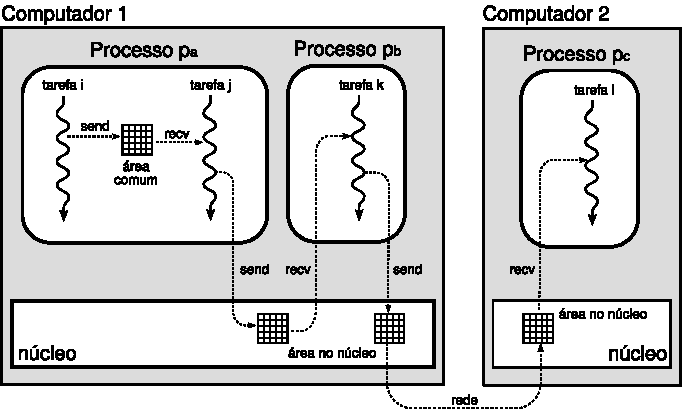
\includegraphics[width=12cm]{exemplo-figura.pdf}
\caption{Comunicação inter-processos.}
\label{fig:comun-intra-inter}
\end{figure}


%=====================================================

\subsection{Exemplo de tabela}

Tabelas são elementos importantes de um documento. No \LaTeX\ as tabelas podem ser objetos flutuantes (definidas no ambiente \texttt{table} e referenciadas por números usando \texttt{label} e \texttt{ref}) ou objetos fixos simples, criados pelo ambiente \texttt{tabular}. A tabela \ref{tab:modelos} é um exemplo de tabela flutuante, cuja posição no texto pode variar em função das quebras de página.

\begin{table}[!htp]
\centering
\caption{Os 16 modelos centrais do UCON$_{\mathrm{ABC}}$}
\label{tab:modelos}
\begin{tabular}{|c|cccc|}
\cline{2-5}
\multicolumn{1}{c|}{}& 0 (imutável) & 1 (\emph{pre-update}) & 2 (\emph{on-update}) & 3 (\emph{pos-update}) \\
\hline
\texttt{preA} & \textbullet & \textbullet & -- & \textbullet \\
\hline
\texttt{onA} & \textbullet & \textbullet & \textbullet & \textbullet \\
\hline
\texttt{preB} & \textbullet & \textbullet & -- & \textbullet \\
\hline
\texttt{onB} & \textbullet & \textbullet & \textbullet & \textbullet \\
\hline
\texttt{preC} & \textbullet & -- & -- & -- \\
\hline
\texttt{onC} & \textbullet & -- & -- & -- \\
\hline
\end{tabular}
\end{table}

%=====================================================

\subsection{Exemplo de fórmula}

Equações destacadas devem ser numeradas como mostra a equação \ref{eq:relatividade}:

\begin{equation}
E = m \times c^2
\label{eq:relatividade}
\end{equation}

%=====================================================

\subsection{Exemplos de código-fonte}

Códigos-fonte podem ser produzidos de forma simples através do ambiente \texttt{verbatim}, como mostra este exemplo:

\begin{footnotesize}
\begin{verbatim}
#include <stdio.h>

int main (int argc, char *argv[])
{
   int i ;                           // uma variavel local

   for (i=0; i< 100; i++)            // um laço for
      printf ("i vale %d\n", i) ;    // uma saída na tela
}
\end{verbatim}
\end{footnotesize}

No entanto, é preferível usar pacotes especializados para a edição ou inclusão de códigos-fonte, como o pacote \texttt{listings}. Eis um exemplo de código-fonte escrito com esse pacote:

% exemplo de código-fonte definido no próprio texto

\begin{lstlisting}
#include <stdio.h>

int main (int argc, char *argv[])
{
   int i ;                           // uma variável local

   for (i=0; i< 100; i++)            // um laço for
      printf ("i vale %d\n", i) ;    // uma saída na tela
}
\end{lstlisting}

Esse pacote também permite incluir códigos-fonte de arquivos externos. Eis um exemplo:

% exemplo de código-fonte incluso

\lstinputlisting{2-fundam/exemplo.c}

%=====================================================

\subsection{Exemplo de algoritmo}

Os pacotes \texttt{algorithm} e \texttt{algorithmic} permitem formatar algoritmos facilmente. Eis um exemplo:

\begin{algorithm}[H]
\caption{Ações de $s_i$ ao encerrar um ciclo:}
\label{alg:on-period-ending}
\begin{small}
\begin{algorithmic}[1]
\FORALL{$x \in \mathcal{K}_i$}
  \STATE{$\mathit{banned}_i(x) \gets$ FALSE}
  \STATE{$mi_i(x) \gets 0$}
  \STATE{$mm_i(x) \gets 0$}
  \STATE{$\mathit{age}_i(x) \gets \mathit{age}_i(x) + 1$}
  \IF{$\mathit{age}_i(x) = \mathit{age}_\mathit{max}$}
     \STATE{$\mathcal{K}_i \gets \mathcal{K}_i - \{x\}$}
     \COMMENT{``esquece'' do servidor $x$}
     \STATE{remove as informações locais sobre $x$}
     \STATE{envia $\mathit{notify}(x,\mathit{undef})$ ao grupo de confiança $\mathcal{T}_i$}
  \ENDIF
\ENDFOR
\end{algorithmic}
\end{small}
\end{algorithm}
 
%=====================================================

\subsection{Exemplos de citação}

Citação curta (só um parágrafo): como afirmou Maquiavel em seu livro \emph{O Príncipe}:

\begin{quote}
``Nada é mais difícil de instituir, mais perigoso de conduzir, mais incerto no seu sucesso, do que liderar a introdução de uma nova ordem de coisas... O inovador faz inimigos em todos aqueles que prosperavam sobre as antigas regras, e somente tíbio suporte é esperado daqueles que prosperariam na novidade, porque os homens são geralmente incrédulos, nunca realmente confiam nas coisas novas, a menos que as tenham testado em experiência''.
\end{quote}

Citação longa (mais de um parágrafo): como afirmou Maquiavel em seu livro \emph{O Príncipe}:

\begin{quotation}
``Nada é mais difícil de instituir, mais perigoso de conduzir, mais incerto no seu sucesso, do que liderar a introdução de uma nova ordem de coisas...

O inovador faz inimigos em todos aqueles que prosperavam sobre as antigas regras, e somente tíbio suporte é esperado daqueles que prosperariam na novidade, porque os homens são geralmente incrédulos, nunca realmente confiam nas coisas novas, a menos que as tenham testado em experiência''.
\end{quotation}

%=====================================================

\section{Uma seção}

\subsection{Uma subseção}

\subsubsection{Uma subsubseção}

%=====================================================

\section{Conclusão}

Todo capítulo (com exceção da introdução e da conclusão) deve encerrar com uma pequena conclusão local, resumindo os tópicos apresentados no capítulo e preparando o leitor para o próximo capítulo (exceto se esse for a conclusão geral). Caso o capítulo tenha apresentado resultados obtidos pelo próprio autor, estes devem ser sucintamente relembrados aqui.

%=====================================================
